%%
%% This is file `tikzposter-template.tex',
%% generated with the docstrip utility.
%%
%% The original source files were:
%%
%% tikzposter.dtx  (with options: `tikzposter-template.tex')
%% 
%% This is a generated file.
%% 
%% Copyright (C) 2014 by Pascal Richter, Elena Botoeva, Richard Barnard, and Dirk Surmann
%% 
%% This file may be distributed and/or modified under the
%% conditions of the LaTeX Project Public License, either
%% version 2.0 of this license or (at your option) any later
%% version. The latest version of this license is in:
%% 
%% http://www.latex-project.org/lppl.txt
%% 
%% and version 2.0 or later is part of all distributions of
%% LaTeX version 2013/12/01 or later.
%% 

\documentclass[a1paper,usenames,dvipsnames]{tikzposter} %Options for format can be included here


\usepackage{color}
\usepackage{graphicx}
\usepackage{enumitem}

 %Choose Layout
\definecolor{mygray}{HTML}{CCCCCC}
\definecolorstyle{myColorStyle}{
\colorlet{colorOne}{gray!25}
\colorlet{colorTwo}{gray!20}
\colorlet{colorThree}{gray!40}
}{
% Background Colors
\colorlet{backgroundcolor}{white}
\colorlet{framecolor}{black!30}
% Title Colors
\colorlet{titlefgcolor}{black}
\colorlet{titlebgcolor}{colorOne}
% Block Colors
\colorlet{blocktitlebgcolor}{colorTwo}
\colorlet{blocktitlefgcolor}{black}
\colorlet{blockbodybgcolor}{colorTwo!50}
\colorlet{blockbodyfgcolor}{black}
% Innerblock Colors
\colorlet{innerblocktitlebgcolor}{white}
\colorlet{innerblocktitlefgcolor}{colorTwo}
\colorlet{innerblockbodybgcolor}{white}
\colorlet{innerblockbodyfgcolor}{colorTwo}
% Note colors
\colorlet{notefgcolor}{colorThree}
\colorlet{notebgcolor}{white}
\colorlet{notefrcolor}{white}
}


\usecolorstyle{myColorStyle}
%\usetitlestyle{mytitlestyle}
\useblockstyle{Default}
\usenotestyle{VerticalShading}

 % Title, Author, Institute
\title{Android Bluetooth Credential Store}
\author{Camilla Reis, Dominik Ziegler}
\institute{Graz University of Technology}
\titlegraphic{
\includegraphics[scale=0.1]{graphic/tugraz.png}}

%-----
\makeatletter % added
\definetitlestyle{mytitlestyle}{
    width=\paperwidth, roundedcorners=0, linewidth=0pt, innersep=0.5cm,
    titletotopverticalspace=0mm, titletoblockverticalspace=16mm,
    titlegraphictotitledistance=0.5pt, titletextscale=0.1}
{%
    \coordinate (topleft) at (\titleposleft,\titlepostop);
    \coordinate (topright) at (\titleposright,\titlepostop);
    \coordinate (lefttoright) at (\titlewidth,0);
    \coordinate (head) at (0,\titlepostop-\titleposbottom);
    %
    \draw[draw=none, left color=blocktitlebgcolor!90!black, right color=titlebgcolor!95]%
        (topright) -- (topleft) -- %
        ($(topleft) - (head)-(0,6)$) .. controls %
        ($(topleft) - (head)-(0,6) + 0.25*(lefttoright) + (0,9)$) and %
        ($(topright) - (head) - 0.5*(lefttoright) - (-10,16)$) .. %
        ($(topright) - (head)$) -- cycle;
%     %
    \draw[draw=none, left color=blocktitlebgcolor, right color=white] %
        ($(topleft) - (head)-(0,2)$) .. controls %
        ($(topleft) - (head)-(-6,3) + 0.25*(lefttoright) + (0,10)$) and ($(topright) -
        (head) - 0.25*(lefttoright) - (-6,17)$).. %
        ($(topright) - (head)$) .. controls %
        ($(topright) - (head) - 0.25*(lefttoright)-(-7,19)$) and %
        ($(topleft) - (head)-(-9,5) + 0.25*(lefttoright) + (0,10)$) .. %
        ($(topleft) - (head)-(0,4)$);
    %
    \draw[draw=none, left color=white, right color=blocktitlebgcolor!90!black]%
        ($(topleft) - (head)-(0,2)$) .. controls %
        ($(topleft) - (head)-(-6,3) + 0.25*(lefttoright) + (0,10)$) and ($(topright) -
        (head)+(0,6) - 0.25*(lefttoright) - (-6,20)$)..%
        ($(topright) - (head)+(0,6)$) -- %
        ($(topright) - (head)$) .. controls %
        ($(topright) - (head) - 0.25*(lefttoright) - (-6,17)$) and %
        ($(topleft) - (head)-(-8,4) + 0.25*(lefttoright) + (0,10)$) .. %
        ($(topleft) - (head)-(0,2)$);
% added the percent character here
    \setlength{\TP@titletoblockverticalspace}{5\TP@titletoblockverticalspace}
}
\makeatother

% make this style active
\usetitlestyle{mytitlestyle}
%-----



\begin{document}

 % Title block with title, author, logo, etc.
\maketitle

%-----------------------------------------

\begin{columns}
\column{0.5}
\block[linewidth=1mm]{Motivation behind the Project}{
Creating a new way to store and handle our passwords and other credentials.\\
Aiming for a safer method of storing personal infomation, than the ones already available. \\
Making credential storage more easy and efficient for the user.}
\column{0.5}
\block[titleright, linewidth=1mm]{Advantages and Goals}{
%\begin{flushright}
Assuring a more secure method of logging into accounts on user's PC or laptop. \\
No reliance on cloud services and secure environment through transfer via Bluetooth. \\
No need for typing in and remembering user credentials. \\
Authentification through fingerprint scanning or master password.
%\end{flushright}
}

\end{columns}
 
 
%-----------------------------------------

 
%\begin{columns}
%\column{0.2}% Width set relative to text width
%\column{0.8}
%\end{columns}

%\block[titlewidthscale=0.6, bodywidthscale=0.8]
%{Variable width title}{Block with smaller width.}

%-----------------------------------------

%\begin{columns}
%\column{0.8}
% expected solutions block
%\column{0.2}
%\end{columns}

%-----------------------------------------

%\begin{columns}
%\column{0.2}
%\column{0.8}
%\block[titleright, linewidth=1mm]{Solution}{sdkfjksdjflk}
%\end{columns}

%-----------------------------------------


\begin{columns}
\column{0.65}

%Grafik-Block
\block[linewidth=1mm]{}
{
\begin{center}
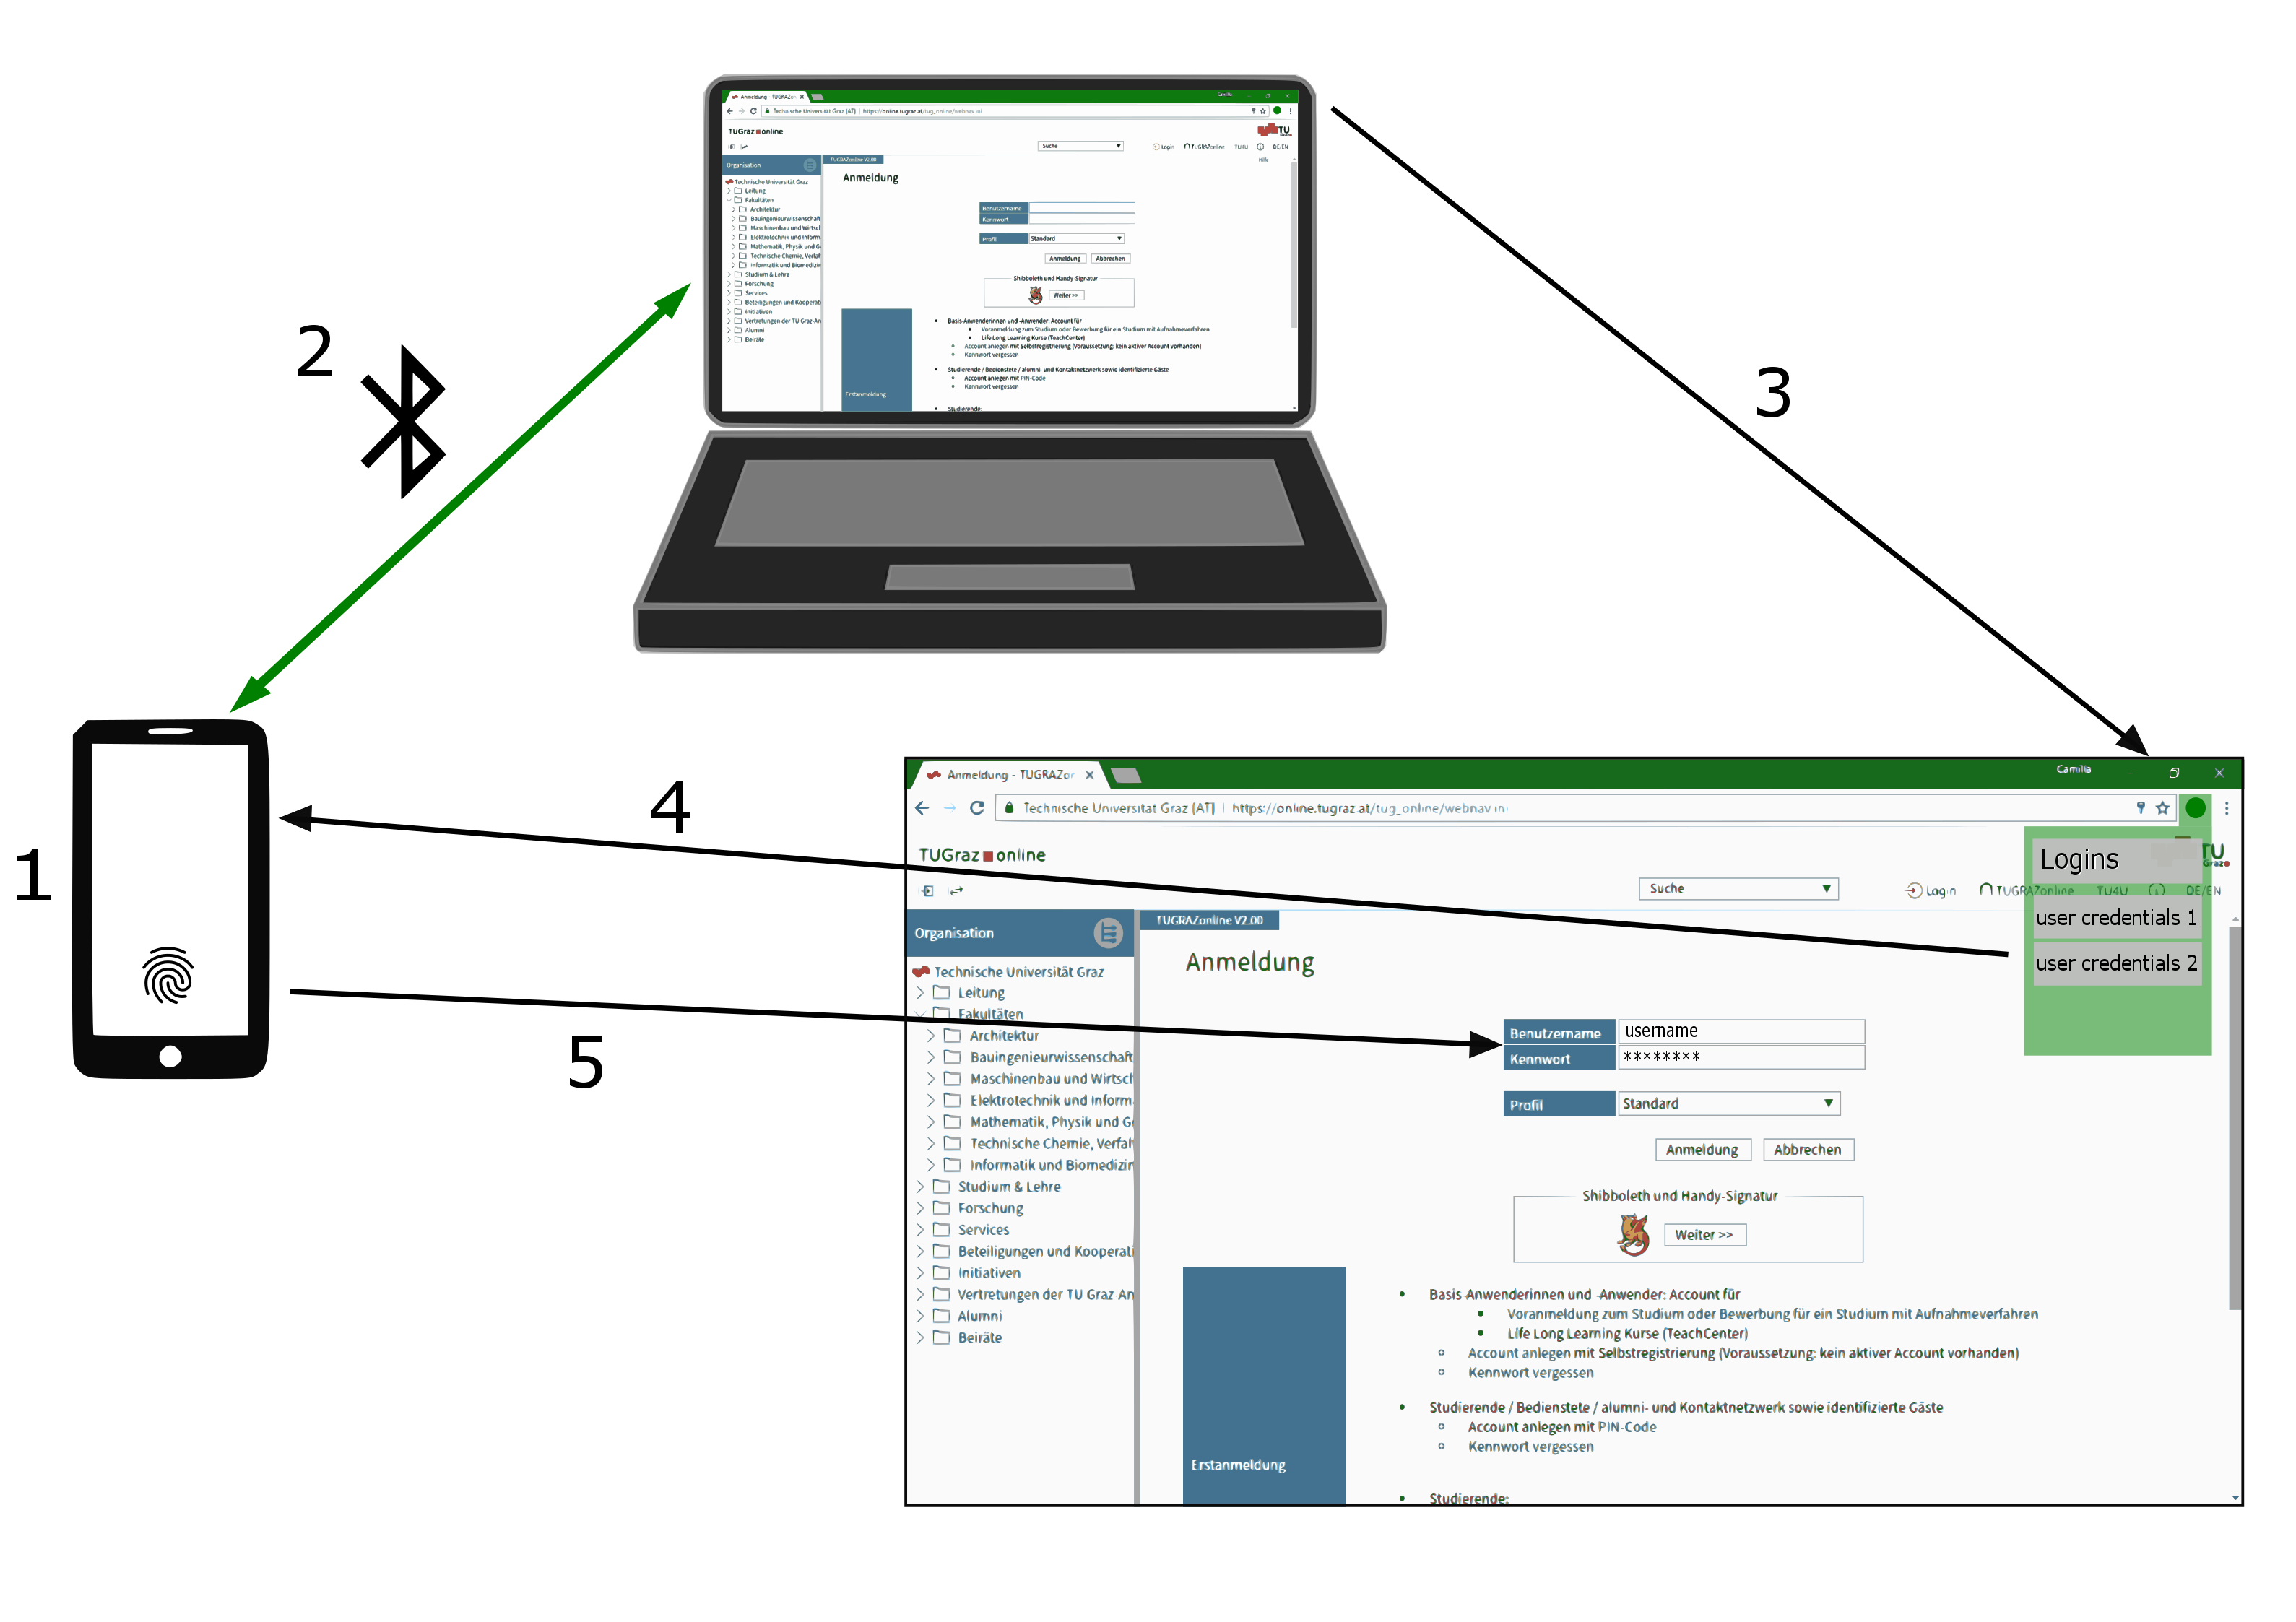
\includegraphics[scale=0.3]{graphic/ablauf.png}
\end{center}
}

\column{0.35}
\block[linewidth=1mm]{Procedure of the Login}{
%\centering
\begin{enumerate}[itemsep=0.0pt, parsep=0.0pt]
\item Saving credentials on device\\
\item Establishing bluetooth connection beween device and browser plug-in \\
\item Checking all available logins for this website \\
\item User selects desired login account \\
\item Authentification at device with fingerprint or master password
\end{enumerate}
}


\end{columns}

\block[titleleft, linewidth=1mm]{Expected Solution}{
We will work with a Bluetooth connection between device and browser plug-in. This gives us a secure environment for transfering the user credentials for the login procedure. \\
Before the credentials are stored in a SQLite database on the device, they are encrypted using a key, which is located in a hardware-backed keystore. This ensures us that the key cannot be retrieved by unauthorized persons or devices for decryption of the data.
}
%weird block
%\block[titleleft, titleoffsetx=2em, titleoffsety=1em, bodyoffsetx=2em,%
% bodyoffsety=-2cm, linewidth=0mm, titlewidthscale=0.7,%
% bodywidthscale=0.9, bodyverticalshift=2cm, titleright]
 
 
 
%\note{Note with default behavior}
%\note[targetoffsetx=12cm, targetoffsety=-1cm, angle=20, rotate=25]
%{Note \\ offset and rotated}

 
%{Block outside of Columns}{Along with several options enabled}

\end{document}



\endinput
%%
%% End of file `tikzposter-template.tex'.
